\section{Esquemático}

\subsection{Insertando componentes y haciendo conexiones}

Primero debemos ubicar los símbolos de los componentes de nustro circuito, \textcolor{red}{\texttt{atajo del teclado: a}}. Se abrirá algo como en la figura \ref{fig:seleccionador_de_simbolo}.

\begin{figure}[H]
	\centering
	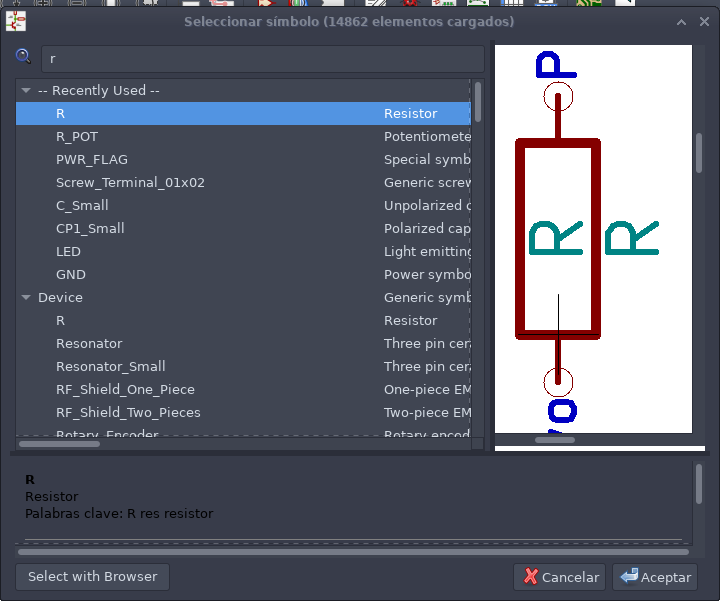
\includegraphics[width=0.5\textwidth]{imagenes/seleccionador_de_simbolo.png}
	\caption{Seleccionador de símbolo, se puede acceder con la tecla ''a''.}
	\label{fig:seleccionador_de_simbolo}
\end{figure}


Podemos buscar por nombre. Hay de todo, transistores, integrados, micrcontroladores y los más básicos, resistores, capacitores e inductores, además de muchísimos más.\\

Para manipular los componentes se puede realizar utilizando los siguientes atajos:
\begin{itemize}
	\item Mover, \textcolor{red}{\texttt{atajo de teclado: m}}
	\item Copiar, \textcolor{red}{\texttt{atajo de teclado: c}}
	\item Rotar, \textcolor{red}{\texttt{atajo de teclado: r}}
	\item Espejar verticalmente, \textcolor{red}{\texttt{atajo de teclado: x}}
	\item Espejar horizontalmente, \textcolor{red}{\texttt{atajo de teclado: y}}
	\item Valor del componente, \textcolor{red}{\texttt{atajo de teclado: v}}
\end{itemize}

Una vez que tengamos todos los componentes, podemos unirlos utilizando las herramientas:
\begin{itemize}
	\item Crear una conexión, \textcolor{red}{\texttt{atajo de teclado: w}}
	\item Etiquetas, las del mismo nombre se encuentran conectadas, \textcolor{red}{\texttt{atajo de teclado: l}}
\end{itemize}


Otras herramientas útiles: 
\begin{itemize}
	\item Insertar texto, \textcolor{red}{\texttt{atajo de teclado: t}}
	\item Dibujar líneas. 
\end{itemize}

{\LARGE \textbf{Atención!!!}} Cuando se conecten los componentes con conexiones (herramienta \texttt{w}) debe prestarse especial atención a que queden conectados como en la figura \ref{fig:comparacion_conexiones}.


\begin{figure}[H]
	\centering
	\begin{subfigure}[b]{0.4\textwidth}
		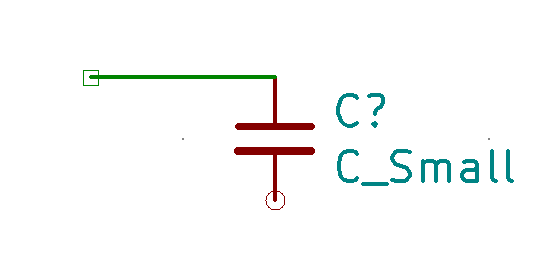
\includegraphics[width=\textwidth]{imagenes/conexion_incorrecta.png}
		\caption{ }
		\label{fig:conexion_incorrecta}
	\end{subfigure}
	\begin{subfigure}[b]{0.4\textwidth}
		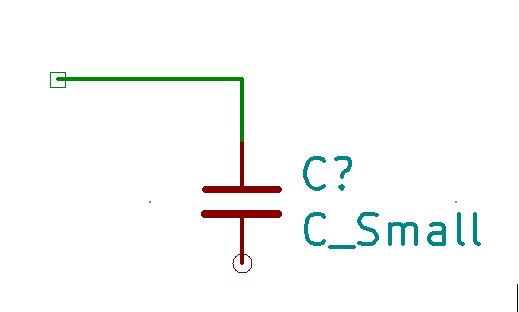
\includegraphics[width=\textwidth]{imagenes/conexion_correcta.png}
		\caption{ }
		\label{fig:conexion_correcta}
	\end{subfigure}
	\caption{El programa puede no reconocer la conexión en la figura \ref{fig:conexion_incorrecta}. En cambio en la conexión de la figura \ref{fig:conexion_correcta} no quedan dudas. }
	\label{fig:comparacion_conexiones}
\end{figure}

\subsection{Anotación y reglas eléctricas}

El Netlist es un archivo que indica qué terminales de qué componentes se encuentran conectados entre sí. Para que pueda diferenciar dos componentes del mismo tipo (para nosotros es fácil, miramos el dibujo en la pantalla y listo) estos deben encontrarse \textbf{enumerados}. Se puede hacer con el símbolo 
\includegraphics[scale=0.5]{imagenes/herramienta_enumerar.png}. En la figura \ref{fig:sin_anotar} se muestra como se ven los componentes sin anotar.

\begin{figure}[H]
	\centering
	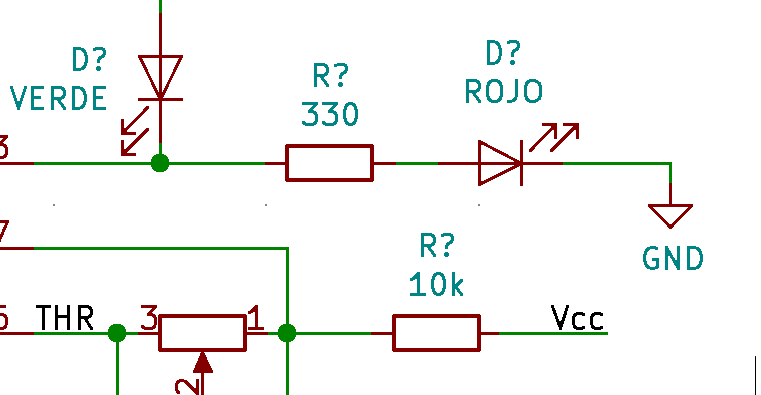
\includegraphics[width=0.5\textwidth]{imagenes/sin_anotar.png}
	\caption{Los componentes tienen sus valores y letras asociadas. El signo de pregunta indica que no se encuentran numeradas y el programa no puede diferenciar, por ejemplo, una resistencia de otra.}
	\label{fig:sin_anotar}
\end{figure}


Luego de anotados los componentes, se obtiene le resultado de la figura \ref{fig:anotados}.

\begin{figure}[H]
	\centering
	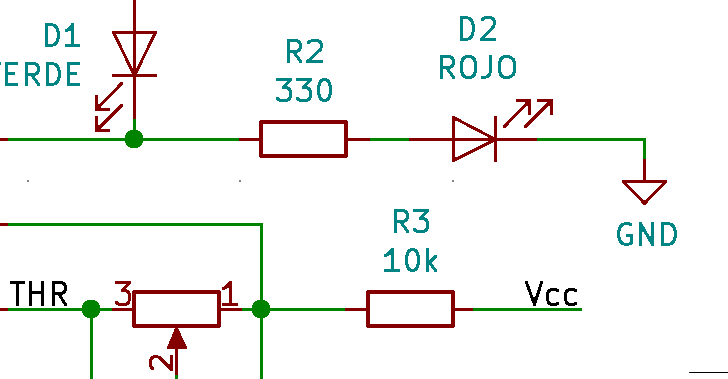
\includegraphics[width=0.5\textwidth]{imagenes/anotado.png}
	\caption{Luego de utilizar la herramienta de anotación, los componentes están numerados y pueden diferenciarse.}
	\label{fig:anotados}
\end{figure}

Una vez que están anotados pasamos a la herramienta de chequeo de conexiones eléctricas (\textbf{Electrical Rules Check, ERC}). Podemos abrirla en el ícono 
\includegraphics[scale=0.5]{imagenes/erc.png}. Nos marcará ciertos problemas como por ejemplo, que no encuentra alimentación en nuestro circuito o que hay terminales de componentes sin conectar. Podemos marcar explícitamente que un pin no va conectado a ningún lado utilizando la herramienta \textbf{no connection}, \textcolor{red}{\texttt{atajo de teclado q}}. 